\section{Target System}
The RG-E Double-Target system utilizes a combination of the JLab/CLAS12
cryotarget and various solid material targets, as shown in Fig. \ref{fig:rge-target}. RG-E will use the following targets in the double-target system:
\begin{itemize}
    \item Liquid:
    \begin{itemize}
        \item Deuterium
        \item Hydrogen
    \end{itemize}
    \item Solid:
    \begin{itemize}
        \item Carbon 12
        \item Aluminum 27
        \item Copper 63
        \item Tin 120
        \item Lead 208
    \end{itemize}
\end{itemize}

  The cryotarget consists of a 2 cm long cell filled with either deuterium or hydrogen. The solid targets are affixed to a specialized flexible band. The solid targets can be interchanged during different run periods using a piezo-motor device to position them with high precision in the beam and aligned with the cryotarget. Only one solid target can be in the beam at the same time.
  The solid target system is enclosed within a vacuum vessel along with the cryogenic system. Surrounding the target system area is a scattering chamber constructed from 1.2 mm thick carbon fiber. Aluminum windows are utilized at the liquid cell's entrance and exit, as well as at the scattering chamber's exit.
  \begin{figure}
      \centering
      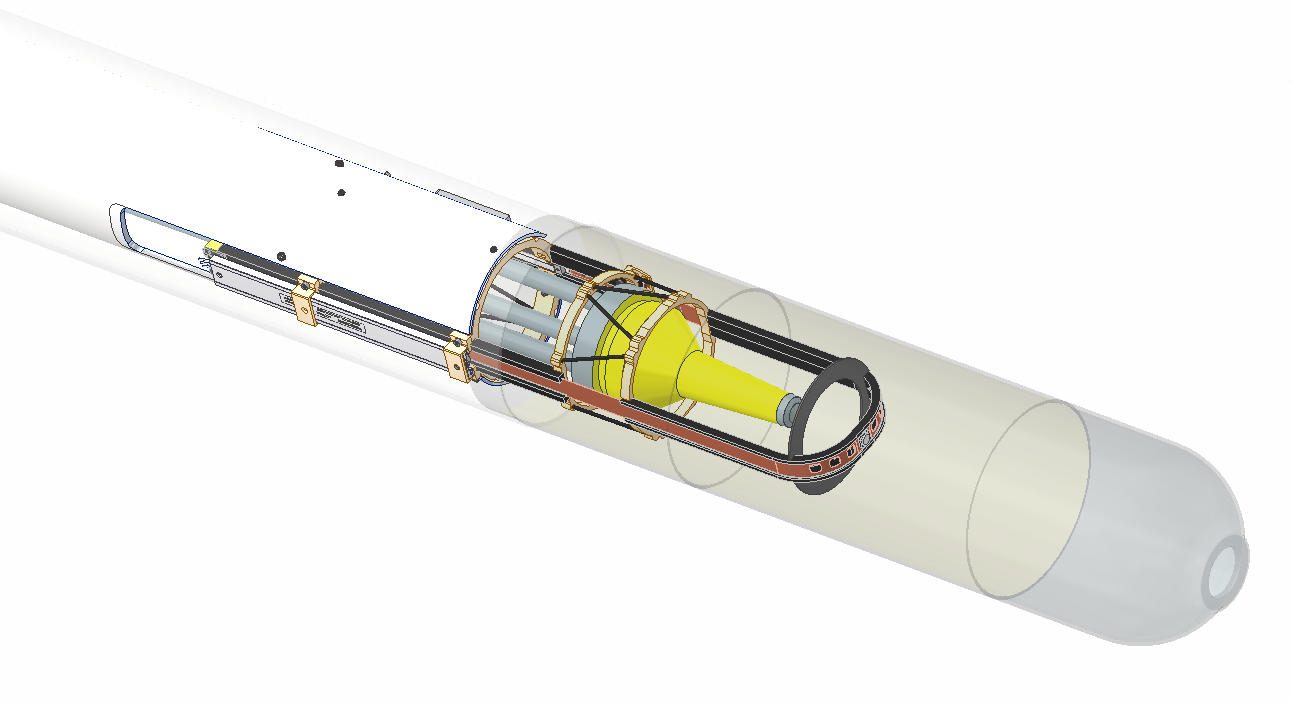
\includegraphics[width=0.9\columnwidth]{pics/rge-target.png}
      \caption{The RG-E Double-Target system. The cryocell system is shown in yellow, and the solid targets are mounted in the flexible band shown in orange. The system is enclosed in a carbon fiber scattering chamber, shown semi-transparent.}
      \label{fig:rge-target}
  \end{figure}

  \subsection{Hazards} 

The cryogenic target contains a condensed cryogenic fluid and is considered a pressure vessel. Sudden warming of the target due to a vacuum breach could result in rapid expansion of the target fluid. The system is designed to safely vent the excess pressure. Failure of the carbon fiber scattering chamber, or the thin window of the scattering chamber could produce a loud noise and could result in a failure of the target integrity.

The target utilizes flammable gas (deuterium or hydrogen) during operation. Failure of the system could release flammable gas into the hall. The target gases and the helium used in the target refrigerator are potential ODH risks, and failure of either system could reduce the oxygen levels in the hall.

The target cell system is protected by 15 psi relief valves.  The target operates in a vacuum chamber, so the total pressure difference possible across the cell is 15~psi~+~14.7 ~psi=~29.7~psi. The cell is considered a pressure vessel. If the Kapton cell ruptures, the target gas would vent into the target vacuum space and the vacuum pumps would turn off. If the vacuum space pressure increases to 1 psi, the target gas will go out of the vacuum space relief valve and be discharged out of the Hall. No target gas would enter the Hall.

\subsection{Mitigations}

The design and construction of the entire Hall B cryo target is in accordance with AMSE standards. During operation, the carbon fiber scattering chamber, and the thin window are surrounded by the Hall-B CLAS12 Central Detectors and are therefore difficult to access.~A protective shield will be placed around the scattering chamber whenever the target is retracted from the Central Detector system and is under vacuum.  Personnel working near the target shall wear hearing and eye protection whenever the carbon fiber extension and window are exposed and the system is under vacuum. No cold cryogenic components are accessible by personnel.

Any work on this system must be covered by ePAS Permit to work(s) (PTW).

Relief valves are installed in all the target pressure circuits so the safety system is entirely passive.~The quantity of flammable gas (H2) is less than 80~g and is therefore considered a class-O installation (!600~g) and the rules and regulations for this installation shall be followed, notably:

\begin{itemize}
\item The area shall be posted ``Danger Flammable Gases. No Ignition Sources" 
\item Combustibles and ignition sources shall be minimized within 10 ft or 3~m of target’s gas handling equipment and piping.
\end{itemize}

The target does not operate in a confined space, and the total quantity of hydrogen/helium in the system is under 1000 standard liters. This presents a negligible oxygen deficiency risk in Hall B and therefore is a class-0 ODH installation.  Hydrogen shall be loaded into the system by qualified personnel only, and those personnel shall follow approved operational gas handling procedures.

The target control software includes numerous alarms (temperature, pressure, vacuum, heater power, etc.) to alert users to potential problems, for both the liquid and solid target systems.

\subsection{Responsible Personnel}

The cryogenic target system will be maintained by Hall B, with support from the JLab Target Group.   The solid target system, specific to RG-E, will be maintained by collaborators from Universidad T\'{e}cnica Federico Santa Mar\'{i}a (UTFSM).

\begin{table}[!htb]
\centering
\begin{tabular}{|c|c|c|c|c|}
\hline
 Name&Department.&Phone&email&Comments \\ \hline
Cryotarget On-Call & Hall B &(757) 218-2266& &1st contact \\ \hline
Xiangdong Wei & Hall B &(516) 635-1957&\href{mailto:xwei@jlab.org}{\nolinkurl{xwei@jlab.org}} &2nd contact \\ \hline
\end{tabular}
\caption{Personnel responsible for the CLAS12 cryotarget system.} 
\label{tb:target}
\end{table}

\begin{table}[!htb]
\centering
\begin{tabular}{|c|c|c|c|c|}
\hline
 Name&Department.&Phone&email&Comments \\ \hline
Solid Target On-Call & &(757) 344-1848 & &1st contact \\ \hline
Hayk Hakobyan & UTFSM & &\href{mailto:hayk@jlab.org}{\nolinkurl{hayk@jlab.org}} &2nd contact \\ \hline
\end{tabular}
\caption{Personnel responsible for the RG-E solid target system.} 
\label{tb:starget}
\end{table}
